\scanpage{21}
On trouve
\[
u_\omega(c_{D_t})=c_{D_t}+d^1_{\underline{\omega}/S}(\underline{\omega})
\]
et plus généralement
\[
\boxed{u_\omega(c)=c+d^1_{\underline{\omega}/S}(\underline{\omega})}
\]
\margin{si $c$ \uline{connexion projective}}

Cela montre

a) $u_\omega(c)$ n'est une connexion projective que si $2\omega=0$ i.e. (si $2$ inv. sur $S$) si $\omega=0$ : donc \deleted{\unsure{pas}} \inserted{même pas} deux connexions projectives différentes ne peuvent donner lieu à des $\unsure{\xi|\zeta}$-fibrés isomorphes.

b) On n'a $u_\omega(c)=c$ que si $d^1_{\underline{\omega}/S}(\underline{\omega})=0$, donc a fortiori $2\omega=0$ donc (si $2$ inv.) $\omega=0$, donc il n'y a pas de $\unsure{\xi|\zeta}$-autom. du \deleted{$\unsure{\xi}$} $\unsure{\xi|\zeta}$-fibré en droites projectives associé à une conn. proj. sur $X$ propre lisse sur $S$ à fibres géom connexes de genre $g\geq2$.

\margin{question : y en a-t-il \unsure{qui ait des sections} horizontales ?}
\figure{\begin{tikzpicture}[x=1cm,y=1cm]
\draw[->] (0,2.4) .. controls (-.25,1.6) and (0,.6) .. (.85,0);
\end{tikzpicture}}
\figure{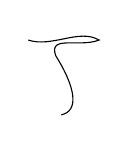
\begin{tikzpicture}[x=1cm,y=1cm]
\draw (0,.55) .. controls (.3,.45) and (.65,.7) .. (.9,.55) .. controls (.65,.45) and (.25,.62) .. (.35,.35) .. controls (.6,-.05) and (.65,-.35) .. (.42,-.4);
\end{tikzpicture}}

\deleted{\unsure{Reprenons} l'\unsure{interprétation} transcendante, et situons donc}
\deleted{\diagram{\begin{tikzcd}
M_g(X) \arrow[dr] & & \operatorname{Conn}(X) \arrow[dl] \\
& M^{\unsure{\xi|\zeta}}_g(X) &
\end{tikzcd}}}

Non, car s'il y en avait, le $\unsure{\xi|\zeta}$-fibré serait associé à un $\unsure{\xi|\zeta}$-fibré affine, donc serait isomorphe à un $P(F)$, où $F$ est une $\unsure{\xi|\zeta}$-extension
\diagram{\begin{tikzcd}
0 \arrow[r,dash] & M \arrow[r] & F \arrow[r] & \mathcal O_X \arrow[r] & 0
\end{tikzcd}}
$M$ est un $\unsure{\xi|\zeta}$-faisceau lin. On aurait donc $E\simeq F\otimes L$, et $\deleted{\unsure{\det}}E\simeq$
% archive foliation: 20
